\documentclass[12pt,a4paper]{scrreprt}
\usepackage{scrhack}

% Textkodierung Deutsch
\usepackage[ngerman]{babel}
\usepackage[T1]{fontenc}
\usepackage[utf8]{inputenc}
\usepackage{lmodern}
\usepackage{xspace}

% Basisinfos
\title{Modellbasierte Testautomatisierung eines verteilen, adaptiven Load-Balancing-Systems}
\author{Gerald Siegert}
\date{\today}
%Variablen welche innerhalb der gesamten Arbeit zur Verfügung stehen sollen
\newcommand{\titleDocument}{Masterarbeit}
\newcommand{\subjectDocument}{im Studiengang Informatik}
\newcommand{\zB}{z.\,B. }
\newcommand{\uA}{u.\,A. }
\newcommand{\sS}{S\# }
\newcommand{\cS}{C\# }
\newcommand{\uU}{u. U.}
\newcommand{\isse}{Institute for Software \& Systems Engineering}

%hier müssen alle Wörter rein, welche Latex von sich auch nicht korrekt trennt bzw. bei denen man die genaue Trennung vorgeben möchte
\hyphenation
{
    Film-pro-du-zen-ten
    Lux-em-burg
    Soft-ware-bau-steins
    zeit-in-ten-siv
}
\renewcommand{\texttt}[1]{%
    \begingroup
    \ttfamily
    \begingroup\lccode`~=`/\lowercase{\endgroup\def~}{/\discretionary{}{}{}}%
    \begingroup\lccode`~=`[\lowercase{\endgroup\def~}{[\discretionary{}{}{}}%
    \begingroup\lccode`~=`.\lowercase{\endgroup\def~}{.\discretionary{}{}{}}%
    \catcode`/=\active\catcode`[=\active\catcode`.=\active
    \scantokens{#1\noexpand}%
    \endgroup
}

% Seitenränder
\usepackage{geometry}
\geometry{left=35mm, right=20mm, top=25mm, bottom=20mm}

% Kopf/Fußzeilen
\usepackage[headsepline]{scrpage2}
\clearscrheadfoot
\pagestyle{scrheadings}

\ihead{\headmark}
\automark{chapter}
\ohead{\pagemark}
\cfoot[\pagemark]{}

\renewcommand*{\headfont}{\normalfont}
\setlength{\headheight}{1.5\baselineskip}

% Grafiken
\usepackage{graphicx}
\usepackage{wrapfig}
\usepackage[format=plain]{caption}

% Textfarben
\usepackage{xcolor}

% Abkürzungen
\usepackage[nohyperlinks,printonlyused]{acronym}

% Zeilenabstand
\usepackage[onehalfspacing]{setspace}
\usepackage{enumitem}
\setlist[itemize]{noitemsep}

% Literatur
\usepackage[style=numeric-comp,natbib=true,maxitems=1,backend=biber,sorting=none]{biblatex}
\usepackage[autostyle=true,german=quotes]{csquotes}
\addbibresource{./literatur.bib}
\addbibresource{./web.bib}
\addbibresource{./abbildungen.bib}

% Listings
\usepackage{listings}
\makeatletter
\definecolor{darkgreen}{rgb}{0,0.5,0}
\lstdefinestyle{base}{
    basicstyle=\footnotesize\ttfamily,
    frame=single,
    numbers=left,
    numberstyle=\tiny,
    breaklines=true,
    tabsize=2,
    captionpos=b,
}
\lstdefinestyle{cs}{
    language=[sharp]c,
    style=base,
    commentstyle=\color{darkgreen},
    keywordstyle=\color{blue},
    morekeywords={ nameof },
}
\lstdefinestyle{plain}{
    language={},
    style=base,
    tabsize=4,
    captionpos=t,
}
% Json Listings
\newcommand\JSONnumbervaluestyle{\color{blue}}
\newcommand\JSONstringvaluestyle{\color{red}}
% switch used as state variable
\newif\ifcolonfoundonthisline
\lstdefinestyle{json}
{
    style=base,
    captionpos=t,
    showstringspaces    = false,
    keywords            = {false,true},
    alsoletter          = 0123456789.,
    morestring          = [s]{"}{"},
    stringstyle         = \ifcolonfoundonthisline\JSONstringvaluestyle\fi,
    MoreSelectCharTable =%
    \lst@DefSaveDef{`:}\colon@json{\processColon@json},
    basicstyle          = \ttfamily,
    keywordstyle        = \ttfamily\bfseries,
}
% flip the switch if a colon is found in Pmode
\newcommand\processColon@json{%
    \colon@json%
    \ifnum\lst@mode=\lst@Pmode%
    \global\colonfoundonthislinetrue%
    \fi
}
\lst@AddToHook{Output}{%
    \ifcolonfoundonthisline%
    \ifnum\lst@mode=\lst@Pmode%
    \def\lst@thestyle{\JSONnumbervaluestyle}%
    \fi
    \fi
    %override by keyword style if a keyword is detected!
    \lsthk@DetectKeywords% 
}
% reset the switch at the end of line
\lst@AddToHook{EOL}%
{\global\colonfoundonthislinefalse}
%%%%%%%%%% end listings

% Verzeichnisse
\makeatletter
\renewcommand\listoffigures{%
    \section*{\listfigurename}\addcontentsline{toc}{section}{\listfigurename}%
    \@mkboth{\MakeUppercase\listfigurename}%
    {\listfigurename}%
    \@starttoc{lof}%
}
\renewcommand\listoftables{%
    \section*{\listtablename}\addcontentsline{toc}{section}{\listtablename}%
    \@mkboth{\MakeUppercase\listtablename}%
    {\listtablename}%
    \@starttoc{lot}%
}
\renewcommand\lstlistoflistings{%
    \section*{\lstlistlistingname}\addcontentsline{toc}{section}{\lstlistlistingname}%
    \@mkboth{\MakeUppercase\lstlistlistingname}%
    {\lstlistlistingname}%
    \@starttoc{lol}%
}
\makeatother

% Hurenkinder, Schusterjungen
\clubpenalty = 10000
\widowpenalty = 10000
\displaywidowpenalty = 10000 

% Referenzen
\usepackage[bookmarksnumbered]{hyperref}

\begin{document}
    % Titelseite
    \setcounter{page}{-100}
    \begin{titlepage}
        \begin{doublespace}
            \thispagestyle{empty}

\begin{figure}[t]
\centering
% \includegraphics[width=0.6\textwidth]{abb/logo1}
~~~~~~~~~~
% \includegraphics[width=0.3\textwidth]{abb/logo2}
\end{figure}


\begin{verbatim}


\end{verbatim}

\begin{center}
\Large{Universität Augsburg}\\
\end{center}


\begin{center}
\Large{Fakultät für Angewandte Informatik}
\end{center}
\begin{verbatim}




\end{verbatim}
\begin{center}
\doublespacing
\textbf{\LARGE{Masterarbeit}}\\
\singlespacing
\begin{verbatim}

\end{verbatim}
\textbf{{~im Studiengang Informatik~}}
\end{center}
\begin{verbatim}

\end{verbatim}
\begin{center}

\end{center}
\begin{verbatim}

\end{verbatim}
\begin{center}
\textbf{zur Erlangung des akademischen Grades \\\ \\ Master of Science}
\end{center}
\begin{verbatim}






\end{verbatim}
\begin{flushleft}
\begin{tabular}{llll}
\textbf{Thema:} & & <Thema der Arbeit> & \\
& & \\
\textbf{Autor:} & & Gerald Siegert & \\
& & MatNr. 1450117 & \\
& & \\
\textbf{Version vom:} & & \today &\\
& & \\
\textbf{Betreuer:} & & M.Sc. Benedikt Eberhardinger &\\
\textbf{1. Prüfer:} & & Prof. Dr. X &\\
\textbf{2. Prüfer:} & & Prof. Dr. Y &\\
\end{tabular}
\end{flushleft}
        \end{doublespace}
    \end{titlepage}
    
    % Abstract
    \pagenumbering{Roman}
    \begin{abstract}
    Durch eine Automatisierung von Tests lassen sich im Bereich der Softwareentwicklung hohe Kosten einsparen.
    Daher wurden zahlreiche Test"=Frameworks und Möglichkeiten zum Testen von Systemen und ihrer Software entwickelt.
    Ein solches Framework ist \acrshort{ss} (\acrlong{ss}), mit dem mithilfe eines modellbasierten Ansatzes Systeme getestet werden können.
    Mithilfe des \acrshort{ss}"=Frameworks soll nun ein Testsystem entwickelt werden, um hiermit automatisiert ein verteiltes, adaptives Load"=Balancing"=System zu testen.
    Hierfür wurde Apache Hadoop ausgewählt, welches mit einer selbstadaptiven Komponente ergänzt wird.
    Diese selbstadaptive Komponente verändert dynamisch und basierend auf den derzeit auf dem Hadoop"=Cluster ausgeführten Anwendungen einige der sonst statischen Einstellungen von Hadoop, womit die verfügbaren Ressourcen des Clusters optimaler genutzt werden können.
    
    Um Hadoop testen zu können, wurde zunächst mithilfe von \acrshort{ss} ein Modell entwickelt, welches die wesentlichen Komponenten des \acrshort{YARN}"=Frameworks von Hadoop abbildet.
    Dieses Modell wurde wiederum mithilfe eines hierfür entwickelten Treibers mit einem realen Hadoop"=Cluster verbunden.
    Dadurch wurde es ermöglicht, durch die Testausführung mit \acrshort{ss} unterschiedliche Anwendungen auf dem realen Cluster auszuführen und die Daten der Anwendungen und des Clusters im Modell zu nutzen.
    Um zu testen, ob sich das entwickelte Testsystem zur Testautomatisierung eines verteilten, adaptiven Load"=Balancing"=Systems eignet, wurde hierfür eine Fallstudie durchgeführt.
    
    In dieser Masterarbeit werden der Aufbau und Ablauf der durchgeführten Fallstudie, sowie die Entwicklung und Implementierung des hierfür genutzten Testsystems erläutert.
    Es wird gezeigt, welche Besonderheiten bei der Durchführung und Auswertung der Fallstudie aufgetreten sind, und inwiefern sich das entwickelte, modellbasierte Testsystem zur Testautomatisierung eines verteilten, adaptiven Load"=Balancing"=Systems eignet.
\end{abstract}

\clearpage
\begin{otherlanguage}{english}
\begin{abstract}
    By automating tests, high costs can be saved in software development.
    Therefore, numerous test frameworks and ways to test systems and their software have been developed.
    One such framework is \acrshort{ss} (\acrlong{ss}), which uses a model-based approach to test systems.
    By using the \acrshort{ss} framework, a test system will be developed to automatically test a distributed, adaptive load-balancing system.
    For this, Apache Hadoop was chosen, which is equipped with an adaptive resource manager.
    The manager detect the current usage of the cluster and modify some of Hadoop's otherwise static settings to make a better use of the available resources.
    
    To test hadoop, a \acrshort{ss} model was developed, which contains the essential componentens of the Hadoop \acrshort{YARN} framework.
    To connect the model to a real Hadoop cluster a driver was developed for this purpose.
    This allows \acrshort{ss} to run different applications on the real cluster and detect the state of the running applications and the cluster.
    To determine the developed test system is suitable for the test automation of a distributed, adaptive load-balancing system, a case study was performed.
    
    This master thesis explains the structure and processes of the case study, as well as the development and implementation of the test system used for this purpose.
    It shows the won experiences by performing the case study and shows how the developed, model-based test system is suitable for test automation of a distributed, adaptive load-balancing system.
\end{abstract}
\end{otherlanguage}


    
    % Verzeichnisse
    \newpage
    \begin{singlespace}
        \tableofcontents
        \addchap{Verzeichnisse}

%\renewcommand{\listfigurename}{Abbildungen}
\listoffigures

%\renewcommand{\lstlistlistingname}{Listings}
\lstlistoflistings

%\renewcommand{\listtablename}{Tabellen}
\listoftables

%\section*{Abkürzungen}\addcontentsline{toc}{section}{Abkürzungen}
\addsec{Abkürzungsverzeichnis}%\addcontentsline{toc}{section}{Abkürzungsverzeichnis}
\begin{acronym}[AppMstr]
    \acro{AM}{ApplicationManager}
    \acro{AppMstr}{ApplicationMaster}
    \acro{DCCA}{Deductive Cause-Consequence Analysis}
    \acro{MARP}{\texttt{maximum-am-resource-percent}}
    \acro{MC}{Model Checking}
    \acro{MCr}[MC]{Model Checker}
    \acro{NM}{NodeManager}
    \acro{RM}{ResourceManager}
    \acro{TLS}{Timeline-Server}
\end{acronym}
    \end{singlespace}
    
    % Inhalt    
    \newpage
    \pagenumbering{arabic}
    
    \chapter{Einleitung}
\label{ch:intro}

Im Bereich der Softwaretests wird heutzutage sehr viel mit automatisierten Testverfahren gearbeitet.
Dies ist insofern logisch, als dass diese Testautomatisierung einerseits Aufwand und damit andererseits direkt Kosten einer Software einspart.
Daher gibt es vor allem im Bereich der Komponententests zahlreiche Frameworks, mit denen Tests einfach und automatisiert erstellt bzw. ausgeführt werden können.
Ein Beispiel für ein solches Testframework wäre das \emph{xUnit}"=Framework, zu dem \uA JUnit\footnote{\url{https://junit.org}} für Java und NUnit\footnote{\url{https://nunit.org/}} für .NET zählen.
Dabei werden zunächst einzelne Testfälle erstellt und können im Anschluss mit der jeweils aktuellen Codebasis jederzeit ausgeführt werden.
Automatisierte Tests können auch dazu genutzt werden, um einen einzelnen Test mit verschiedenen Eingaben durchzuführen.
Dadurch können verschiedene Eingabeklassen (wie negative oder positive Ganzzahlen) mit sehr geringem Aufwand in einem Test genutzt werden und somit verschiedene Testfälle direkt ausgeführt werden, wodurch eine massive Kosteneinsparung einhergeht \cite{Polo2013}.

Es gibt aber nicht nur Frameworks für Komponententests, sondern auch für modellbasierte Testverfahren wie \zB dem \ac{MC}.
Beim \ac{MC} wird ein Modell mithilfe eines entsprechenden Frameworks automatisiert auf seine Spezifikation getestet und geprüft, unter welchen Umständen diese verletzt wird \cite{Grumberg1999,Habermaier2015}.

In dieser Masterarbeit soll daher nun ein verteiltes, adaptives Load"=Balancing"=System getestet werden.
Hauptziel ist es, zu ermitteln, wie ein modellbasierter Testansatz auf ein komplexes Beispiel übertragen werden kann.
Dafür wird zunächst ein reales System als vereinfachtes Modell nachgebildet und anschließend mithilfe eines \ac{MC} getestet.
Es soll dabei auch ermittelt werden, wie ein reales System in das Modell eingebunden werden kann und wie bei Problemen mit asynchronen Prozessen innerhalb des verteilten Systems umgegangen werden muss.

\todo{vielleicht Testing MapReduce-Based Systems einbringen?}

    \chapter{Relevante Methodiken}\label{chap:methodiken}

\section{Model Checking}\label{sec:modelchecking}

\ac{MC} ist eine Möglichkeit, um Systeme zu testen und zu verifizieren. Dazu werden vom \ac{MCr} alle möglichen Systemzustände in einem \emph{brute-force}-ähnlichem Vorgehen getestet und somit alle möglichen Szenarien getestet. Die Anzahl der Zustände kann sehr schnell $ 10^{120} $ oder mehr betragen \cite{Grumberg1999,Baier2008}.

\begin{figure}
	\includegraphics{./images/mcSchema.pdf}
	\caption[Schematischer Aufbau beim MC]{Schematischer Aufbau beim MC, nach \cite{Baier2008}}
	\label{fig:mcSchema}
\end{figure}

Ein \ac{MCr} nutzt, wie der Name schon sagt, ein Modell des Systems, um das System zu testen. Wie bei jeder anderen modellbasierten Technik ist daher die Qualität des \ac{MC} nur so gut wie das darauf zugrunde liegende Modell. Ein Modell kann auch als endlicher Automat angesehen werden, da ein Modell ebenfalls eine endliche Anzahl an möglichen Zuständen und dazugehörige Übergänge besitzt. Für jede Eigenschaft eines Zustandes muss zudem mithilfe einer sog. \emph{temporalen Logik}, also mathematisch bzw. formal, festgelegt werden, was gültige Werte dieser Eigenschaft sind. Die dazu benötigten Informationen werden aus den Anforderungen des Systems ermittelt und dem \ac{MCr} übergeben. So können später verschiedene Eigenschaften des gesamten Systems (\zB die formale Korrektheit, die Ausführbarkeit ohne Deadlocks oder die Einhaltung von Sicherheitsvorgaben) geprüft werden.

Zur Ausführung wird das gesamte Modell zunächst initialisiert und dann automatisch und systematisch vom \ac{MCr} auf Fehler und ungültige Zustände geprüft. In der Regel ist aber auch eine Ausführung als reine Simulation des Systems möglich, ohne explizit nach Fehlern zu suchen.

Wenn alle Zustände und deren Eigenschaften die Anforderungen erfüllen, erfüllt auch das Modell die Spezifikation. Wenn ein Zustand bzw. Eigenschaft die Anforderungen nicht erfüllt, prüft der \ac{MCr} anhand eines Gegenbeispiels den Ausführungspfad zum Fehler. Dadurch kann ermittelt werden, wo die Fehlerursache liegt. Einige der wesentlichen Fehlertypen und Ursachen sind:

\begin{description}
	\item[Modelling Error] Der Fehler liegt im Modell, welches korrigiert werden muss.
	\item[Design Error] Der Fehler liegt in den formellen oder informellen Anforderungen, dadurch muss das Modell und/oder die temporale Logik korrigiert werden.
	\item[Property Error] Der Fehler ist wirklich ein Fehler im System, welcher gefunden werden soll.
\end{description}

Möglich ist aber auch, dass die Ressourcen nicht ausreichen, um alle Zustände zu prüfen. In so einem Fall gibt es mehrere Möglichkeiten, damit umzugehen, \zB können Heuristiken oder Abstraktionen vom Modell genutzt werden \cite{Baier2008,Eberhardinger2016}.

\ac{MC} besitzt durch seine Charakteristik einige Vorteile, \uA \cite{Baier2008}:
\begin{itemize}
	\item \ac{MC} ist universell nutzbar, \zB für Software, Hardware oder eingebettete Systeme
	\item Partielle Verifikation ist möglich ohne das gesamte System testen zu müssen
	\item Vollständig automatisierbar und benötigt kaum Benutzerinteraktion oder hohe Expertise
\end{itemize}

Natürlich gibt es aber auch einige Nachteile, \uA \cite{Baier2008}:
\begin{itemize}
	\item Mit \ac{MC} wird nur ein Systemmodell und nicht das eigentliche System getestet, was weitere Fehler nicht ausschließt
	\item Hauptsächlich für steuerungsbasierte Anwendungen und nicht für datenbasierte Anwendungen geeignet
	\item Anzahl der möglichen Zustände kann zu hoch sein, um alle zu testen
\end{itemize}

Es gibt zahlreiche \ac{MC}-Frameworks, die bereits erwähnten \emph{LTSmin} und \emph{\sS} sind nur zwei davon.

\section{\acl{ss}}
\label{sec:ssharp}

\todo{Testen unter SS allgemein genauer erklären und an neue Abschnitte anpassen}
\textbf{\acf{ss}} ist ein am \isse der Universität Augsburg entwickeltes Framework zum Testen und Verifizieren von Systemen und Modellen.
Da es in \cS entwickelt wurde und \cS auch zum Entwickeln von Modellen und dazugehörigen Testszenarien genutzt wird, können zahlreiche Features des .NET"=Frameworks bzw. der Sprache \cS im Speziellen genutzt werden.
\ac{ss} vereint dabei die Simulation, die Visualisierung, modellbasierte Tests sowie die Verifizierung der Modelle durch einen \ac{MCr} \cite{Habermaier2015,Habermaier2016}.
Dadurch können alle Schritte einer vollständigen Analyse inkl. Modellierung direkt im Visual Studio ausgeführt werden und somit auch alle Features der IDE und .NET, wie \zB die Debugging"=Werkzeuge, genutzt werden.
Um entsprechende Analysen zu gewährleisten, hat das Framework jedoch auch einige Einschränkungen, wodurch \zB Schleifen und Rekursionen nur eingeschränkt bzw. nicht möglich sind.
Eine der größten Einschränkungen ist allerdings, dass während der Laufzeit keine neuen Objektinstanzen innerhalb des zu testenden Modells erzeugt werden können, sodass alle benötigten Instanzen bereits während der Initialisierung des Modells erzeugt werden müssen \cite{Habermaier2015}.

\subsection{Aufbau eines Modells}
\label{subsec:ssharpModel}

\todo{Hier Oracle, Modell selbst und so rein}

Um nun ein System testen zu können, muss dieses zunächst mithilfe von \cS-Klassen und -Instanzen modelliert werden.
Die dafür verwendeten Modelle sind meist stark vereinfacht und bilden nur die wesentlichen Aspekte der realen Systeme ab.
Für einen korrekten Test ist es jedoch wichtig, dass das Modell des Systems vergleichbar mit dem echten System ist.

Folgendes Beispiel zeigt den typischen, grundlegenden Aufbau einer \ac{ss}-Komponente:

\begin{lstlisting}[label=lst:ssExample,style=cs,
caption={Grundlegender Aufbau einer \acs{ss}-Komponente.}]
public class MyCOmponent : Component
{
  // fault definition, also possible: n§§ew PermanentFault()
  public readonly Fault MyFault = new TransientFault();
  
  // interaction logic (Fields, Properties, Methods...)
  
  // fault effect
  [FaultEffect(Fault = nameof(MyFault))]
  internal class MyFaultEffect : MyCOmponent
  {
    // fault effect logic
  }
}
\end{lstlisting}

Jede Komponente des Modells muss von \texttt{Component} erben, um als \ac{ss}-Komponente definiert zu sein.
Jede Komponente kann nun temporäre (\texttt{TransientFault}) oder dauerhafte (\texttt{PermanentFault}) Komponentenfehler enthalten, welche zunächst innerhalb der Komponente als Felder definiert werden. 
Der Effekt eines Komponentenfehlers wird anschließend in der entsprechenden Effekt"=Klasse definiert, welche von der Hauptklasse (hier \texttt{YarnNode}) erbt und mithilfe des Attributs \texttt{FaultEffectAttribute} dem dazugehörigen Komponentenfehler zugeordnet wird \cite{Habermaier2016}.

\subsection{Ausführung eines Modells mit \acs{ss}}
\label{subsec:ssharpExecution}

Um die Modelle zu testen, kommen in \ac{ss} verschiedene Werkzeuge zum Einsatz.
Eines davon ist eine reine Simulation, bei der das Framework nur einen Ausführungspfad ausführt und dabei keine Komponentenfehler aktiviert bzw. die Aktivierung \textit{manuell} gesteuert werden kann.
Ein weiterer Nutzen liegt in der Möglichkeit, im ausgeführten Ausführungspfad zeitliche Abläufe zu berücksichtigen, da hier das Modell Schritt für Schritt ausgeführt wird.
Hierbei wird für jede im Modell genutzte Komponente pro Schritt einmal die jeweilige Methode \texttt{Update()} aufgerufen, in der die jeweiligen Komponenten ihre Aktivitäten durchführen \cite{Habermaier2016}.

Ein anderes wichtiges Werkzeug von \ac{ss} ist die \ac{DCCA}, welche eine vollautomatische und \ac{MC}-basierte Sicherheitsanalyse ermöglicht.
Dabei wird selbstständig die Menge der aktivierten Komponentenfehler ermittelt, mit denen das Gesamtsystem nicht mehr rekonfiguriert werden kann und somit ausfällt.
Je nach Konfiguration können dazu auch Heuristiken genutzt werden, welche die Analyse beschleunigen und genauer machen können \cite{Eberhardinger2016}.
Dabei werden die verschiedenen aktivierten Komponentenfehler während der Analyse in tolerierbare und nicht-tolerierbare Fehler unterschieden.
Tolerierbare Komponentenfehler werden dazu genutzt, die Grenzen der Selbstkonfiguration des Systems zu ermitteln.
Dabei wird für jeden Systemzustand nach einer Rekonfiguration durch die \ac{DCCA} eine neue Fehlermenge ermittelt, mit der das System gerade noch lauffähig ist.
Das Auftreten eines tolerierbaren Komponentenfehler ist also gleichbedeutend mit einem einfachen Fehler im System, welcher die gesamte Funktionsweise des Systems nicht massiv einschränkt und eine Rekonfiguration noch ermöglicht.
Sobald jedoch ein Fehler auftritt, durch den eine Rekonfiguration des Systems nicht mehr möglich ist, wurde ein nicht-tolerierbarer Fehler gefunden, durch den das System nicht mehr funktionsfähig ist \cite{Habermaier2015}.

Das dritte Werkzeug zur Ausführung von Modellen in \ac{ss} ist der \ac{MCr} selbst.
Hierbei kann der in \ac{ss} bereits enthaltene, oder alternativ \emph{LTSmin}\footnote{\url{http://ltsmin.utwente.nl/}} genutzt werden \cite{SSWikiModelChecking}.
Beim \ac{MC} werden in einem \emph{brute-force}-ähnlichem Verfahren alle möglichen Zustände und Ausführungspfade in einem Modell mit einer endlichen Anzahl an Zuständen getestet.
Dadurch wird es ermöglicht, verschiedene Eigenschaften eines System zu testen und Fehler (\zB Deadlocks) zu erkennen \cite{Grumberg1999}.

    \chapter{Fallstudie}\label{sec:fallstudie}

\input{./fallstudie/ablauf}

\section{Apache Hadoop}\label{sec:hadoop}

\textbf{Apache Hadoop} ist ein Open-Source-Software-Projekt, mit dessen Hilfe ermöglicht wird, Programme zur Datenverarbeitung mit großen Ressourcenbedarf auf verteilten System auszuführen. Hadoop wird von der \emph{Apache Foundation} entwickelt und bietet verschiedene Komponenten an, welche vollständig skalierbar sind, von einer einfachen Installation auf einem PC bis hin zu einer Installation über mehrere Server in einem Serverzentrum. Hadoop besteht hauptsächlich aus folgenden Kernmodulen \cite{HadoopHomePage}:

\begin{description}
	\item[Hadoop Common] Gemeinsam genutzte Kernkomponenten
	\item[Hadoop YARN] Framework zur Verteilung und Ausführung von Anwendungen und das dazugehörige Ressourcen-Management
	\item[Hadoop Distributed File System] Kurz HDFS, Verteiltes Dateisystem
	\item[Hadoop MapReduce] YARN-Basiertes System zum Verarbeiten von großen Datenmengen
\end{description}

Hadoop ermöglicht es dadurch, sehr einfach mit Anwendungen umzugehen, welche große Datenmengen verarbeiten. Da es für Hadoop nicht relevant ist, auf wie vielen Servern es läuft, kann es beliebig skaliert werden, wodurch entsprechend viele Ressourcen zur Bearbeitung und Speicherung von großen Datenmengen zur Verfügung stehen können.

\begin{figure}
	\centering
	\includegraphics[width=\columnwidth]{./images/yarn_architecture.png}
	\caption[Architektur von YARN]{Architektur von YARN (entnommen aus \cite{HadoopYarnArch271})}
	\label{fig:yarnarch}
\end{figure}

Die Kernidee der Architektur von \textbf{YARN} ist die Trennung vom Ressourcenmanagement und Scheduling. Dazu besitzt der Master bzw. \emph{Controller} den \ac{RM}, welcher für das gesamte System zuständig ist und die Anwendungen im System verteilt und überwacht und somit auch als \emph{Load-Balancer} agiert. Er besteht aus zwei Kernkomponenten, dem \ac{AM} und dem \emph{Scheduler}. Der \ac{AM} ist für die Annahme und Ausführung von einzelnen Anwendungen zuständig, denen der Scheduler die dafür notwendigen Ressourcen im Cluster zuteilt.

Jeder Slave-\emph{Node} im Hadoop-Cluster besitzt einen \ac{NM}, welcher für die Überwachung der Ressourcen des Nodes und der darauf ausgeführten Anwendungs-Container zuständig ist und diese dem \ac{RM} mitteilt.

Jede YARN-Anwendung bzw. Job besteht aus einem oder mehreren Ausführungsversuchen, genannt \emph{Attempts}, denen wiederum mehrere \emph{Container} zugeordnet sind. Container können auf einem beliebigen Node ausgeführt werden und repräsentieren die Ausführung eines Tasks der Anwendung. Ein besonderer Container bildet dabei der \ac{AppMstr}, welcher innerhalb seines Attempts für das anwendungsbezogene Monitoring und die Kommunikation mit dem \ac{RM} und \ac{NM} zuständig ist und die dazu notwendigen Informationen bereit stellt \cite{HadoopYarnArch271}.

Hadoop enthält zudem einen sog. \ac{TLS}. Er ist speziell dafür entwickelt, die Metadaten und Logs der YARN-Anwendungen zu speichern und jederzeit, also auch als Anwendungshistorie, auszugeben \cite{HadoopYarnTlServer271}.

\begin{figure}
    \centering
    \includegraphics[width=.8\columnwidth]{./images/hdfsarchitecture.png}
    \caption[Architektur des HDFS]{Architektur des HDFS (entnommen aus \cite{HadoopHdfsDesc271})}
    \label{fig:hdfsarch}
\end{figure}

Das \textbf{HDFS} basiert auf der gleichen Architektur wie YARN und besitzt ebenfalls einen Master und mehrere Slaves, welches in der Regel die gleichen Nodes sind wie bei YARN sind. Der \emph{NameNode} ist als Master für die Verwaltung des Dateisystems zuständig und reguliert den Zugriff auf die darauf gespeicherten Daten. Die Daten selbst werden in mehrere Blöcke aufgeteilt auf den \emph{DataNodes} gespeichert. Um den Zugriff auf die Daten im Falle eines Node-Ausfalls zu gewährleisten, wird jeder Block auf anderen Nodes repliziert. Dateioperationen (wie Öffnen oder Schließen) werden direkt auf den DataNodes ausgeführt, sie sind darüber hinaus auch dafür verantwortlich, dass Clients die Daten lesen oder beschreiben können \cite{HadoopHdfsDesc271}.

\textbf{MapReduce} bietet analog zu YARN die Möglichkeit, Anwendungen mit einem großen Ressourcenbedarf, welche große Datenmengen verarbeiten, auf einem gesamten Cluster auszuführen. Dazu werden bei einem MapReduce-Job die Eingabedaten aufgeteilt, anschließend von den sog. \emph{Map Tasks} verarbeitet und deren Ausgaben von den sog. \emph{Reduce Tasks} geordnet. Für die Ein- und Ausgabe der Daten wird in der Regel das HDFS, für die Ausführung der einzelnen Tasks YARN genutzt \cite{HadoopMapRedTutorial271}. MapReduce kann auch als Vorgänger von YARN angesehen werden, da YARN auch als \emph{MapReduce Next Gen} bzw. \emph{MRv2} bezeichnet wird und aufgrund der API-Kompatibilität von YARN jede MapReduce-Anwendung in der Regel auch auf YARN ausgeführt werden kann \cite{HadoopYarnArch271,HadoopYarnOverview271}.


\section{Adaptive Komponente in Hadoop}\label{sec:inriaSetting}

Ein normales Hadoop besitzt von Haus aus keine adaptive Komponente, sondern rein statische Einstellungen. Um damit Hadoop zu optimieren, müssen die Einstellungen immer manuell auf den jeweils benötigten Anwendungstyp angepasst werden. Dazu gibt es auch bereits verschiedene Scheduler, den \emph{Fair Scheduler}, welcher alle Anwendungen ausführt und ihnen gleich viele Ressourcen zuteilt, und den \emph{Capacity Scheduler}. Letzterer sorgt dafür, dass nur eine bestimmte Anzahl an Anwendungen pro Benutzter gleichzeitig ausgeführt wird und teilt ihnen so viele Ressourcen zu, wie benötigt werden bzw. der Benutzter nutzen darf. Entwickelt wurde der Capacity Scheduler vor allem für Cluster, die von mehreren Organisationen gemeinsam verwendet werden und sicherstellen soll, dass jede Organisation eine Mindestmenge an Ressourcen zur Verfügung hat \cite{HadoopCapScheduler271}.

Je nach Bedarf besitzt der Capacity Scheduler entsprechende Einstellungen, um \zB den verfügbaren Speicher pro Container festzulegen. Eine weitere Einstellung des Schedulers ist \texttt{maximum-am-resource-percent}, auch MARP genannt, der angibt, wie viele Prozent der gesamten Ressourcen durch \ac{AppMstr} genutzt werden dürfen \cite{HadoopCapScheduler271}. Damit bewirkt diese Einstellung indirekt auch die maximale Anzahl an Anwendungen, die gleichzeitig ausgeführt werden dürfen. Da der MARP-Wert jedoch nicht während der Laufzeit dynamisch angepasst werden kann, haben \citeauthor{zhang2016} in \cite{zhang2016} einen Ansatz zur dynamischen Anpassung des MARP-Wertes zur Laufzeit von Hadoop vorgestellt. Dadurch wird der MARP-Wert abhängig von den ausgeführten Anwendungen adaptiv zur Laufzeit angepasst, sodass immer möglichst viele Anwendungen gleichzeitig ausgeführt werden können. Gemäß \citeauthor{zhang2016} werden dadurch Anwendungen im Schnitt um bis zu 40 \% schneller ausgeführt.

\begin{figure}
    \centering
    \includegraphics[width=.8\columnwidth]{./images/marpValue.pdf}
    \caption[LoJP und LoJT in Hadoop]{LoJP und LoJT in Hadoop \cite{zhang2016}}
    \label{fig:marpValue}
\end{figure}

Der Hintergrund dieser \emph{Selfbalancing-Komponente} ist der, dass durch den MARP-Wert der für die Anwendungen verfügbare Speicher in zwei Teile aufgeteilt wird. Im einen Teil befinden sich alle derzeit ausgeführten \ac{AppMstr}, im anderen Teil die von den Anwendungen benötigten weiteren Container. Wie groß der Teil für die \ac{AppMstr} ist, wird nun durch den MARP-Wert bestimmt. Ist der MARP-Wert zu klein, können nur wenige \ac{AppMstr} (und damit Anwendungen) gleichzeitig ausgeführt werden (\emph{Loss of Jobs Parallelism}, LoJP). Ist der MARP-Wert jedoch zu groß, können für die ausgeführten Anwendungen nur wenige Container bereitgestellt werden, wodurch sich die Ausführung für eine Anwendung wesentlich verlangsamt (\emph{Loss of Job Throughput}, LoJT)\cite{zhang2016}.

Die Selfbalancing-Komponente passt daher den MARP-Wert abhängig von der Speicherauslastung dynamisch zur Laufzeit an. So wird der MARP-Wert verringert, wenn die Speicherauslastung sehr hoch ist, und erhöht, wenn die Speicherauslastung sehr niedrig ist \cite{zhang2016}. Dadurch wird es ermöglicht, dass die maximal mögliche Anzahl an Anwendungen ausgeführt werden kann. Die Evaluation von \citeauthor{zhang2016} ergab zudem, dass die dynamische Anpassung des MARP-Wertes zudem auch effizienter ist als eine manuelle, statische Optimierung.


\section{Umsetzung des realen Clusters}\label{sec:aufbauCluster}

\citeauthor{zhang2016} haben im Rahmen ihrer gesamten Forschungsarbeit die Open"=Source"=Plattform Hadoop"=Benchmark entwickelt und auf Github zur Verfügung gestellt.\footnote{\url{https://github.com/Spirals-Team/hadoop-benchmark}}
Sie wurde speziell zum Einsatz in der Forschung erstellt und kann jederzeit an die eigenen Bedürfnisse angepasst werden.
Auf Basis dieser Plattform und der enthaltenen Benchmarks wurde das reale Cluster für diese Masterarbeit aufgebaut.

\subsection{Plattform Hadoop"=Benchmark}\label{sec:hadoopBenchmark}

Die Plattform ist in mehrere Szenarien unterteilt, darunter ein Hadoop in der Version 2.7.1 ohne Änderungen und ein darauf basierendes Szenario mit der Selfbalancing"=Komponente.
Hadoop"=Benchmark basiert auf der Software \emph{Docker}\footnote{\url{https://www.docker.com/}} und dem dazugehörigen Tool \emph{Docker Machine}, um damit mit wenigen Befehlen ein Hadoop"=Cluster aufbauen zu können.
Mit \emph{Graphite}\footnote{\url{https://graphiteapp.org/}} ist zudem ein Monitoring"=Tool enthalten, mit dem die Systemwerte wie CPU- oder Speicher"=Auslastung des Clusters überwacht und analysiert werden kann.

\begin{figure}
    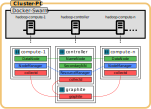
\includegraphics{./images/hadoopBenchmarkArch.png}
    \caption[High"=Level"=Architektur von Hadoop"=Benchmark]
    {High"=Level"=Architektur von Hadoop"=Benchmark.
        Entnommen aus \cite{abb:hadoopBenchmarkArch}.}
    \label{fig:hadoopBenchmarkArchitecture}
\end{figure}

\autoref{fig:hadoopBenchmarkArchitecture} zeigt die grundlegende Architektur der Plattform, die mithilfe eines Docker"=Swarms auf mehreren \emph{Docker Machines} ein Cluster erstellt, auf denen dann in den Docker"=Containern das eigentliche Hadoop"=Cluster ausgeführt wird.
In Hadoop"=Benchmark werden mithilfe von Docker"=Machine und VirtualBox\footnote{\url{https://www.virtualbox.org/}} virtuelle Maschinen erstellt, die mit dem  Betriebssystem \emph{Boot2Docker} ausgestattet sind.
Boot2Docker ist eine leichtgewichtige Linux"=Distribution, auf der Docker bereits vorinstalliert ist \cite{DockerMachineGettingStartedVm}.
Jeder Hadoop"=Container enthält zudem das Tool \emph{collectd}\footnote{\url{https://collectd.org/}}, was das Monitoring des Containers auf Systemebene übernimmt und die Daten an den Graphite"=Container übermittelt.
Dadurch wird es möglich, eine beliebige Anzahl an voneinander unabhängigen Nodes auf einem physischen Computer ausführen zu können.
Auch ist es möglich, den Docker"=Machines einen beliebig großen Arbeitsspeicher zur Verfügung zu stellen.

Die Plattform Hadoop"=Benchmark enthält zudem einige Benchmark"=Anwendungen:

\begin{itemize}
    \item Hadoop Mapreduce Examples
    \item Intel HiBench\footnote{\url{https://github.com/intel-hadoop/HiBench}}
    \item \ac{SWIM} \footnote{\url{https://github.com/SWIMProjectUCB/SWIM}}
\end{itemize}

Eine Besonderheit bildet der SWIM"=Benchmark, welcher sehr Ressourcenintensiv ist und daher auf einem \emph{Single Node Cluster}, also einem kompletten Hadoop"=Cluster auf nur einem Computer, sehr zeitintensiv sein kann.
Der Intel HiBench"=Benchmark besteht aus Kategorien wie \emph{Machine Learning} oder Graphen, welche wiederum aus einen oder mehreren \emph{Workloads} bestehen, welche entsprechende Anwendungen bzw. Algorithmen auf dem Hadoop"=Cluster ausführen.
Einige der Hibench"=Workloads basieren auf den Mapreduce Examples, welche wiederum voneinander unabhängige Beispielanwendungen für Hadoop darstellen.

\subsection{In dieser Fallstudie verwendetes Setup}\label{sec:clusterFallstudie}

Da die Plattform Hadoop"=Benchmark mithilfe von Docker auf einem physischen PC sehr einfach ein komplettes Hadoop"=Cluster ausführen kann, wurde die Plattform für diese Fallstudie als Basis genutzt.
Da Docker und Hadoop vor allem für den Einsatz in einer Linux"=Umgebung entwickelt wurden, werden für die Fallstudie zwei Computer genutzt, auf denen das Cluster wahlweise auf einem oder auf beiden Hosts ausgeführt werden kann.
Zudem wird auf einem Host eine VM mit Windows 10 ausgeführt, das zum Ausführen des .NET"=Frameworks bzw. \sS benötigt wird.
Beide zum Einsatz kommenden Hosts sind jeweils mit einem Intel Core i5"=4570 @ 3,2 GHz x 4, 16 GB Arbeitsspeicher sowie einer SSD ausgestattet, auf der Ubuntu 16.04 LTS installiert ist.
Die Verbindung von Windows zu Linux auf beiden Hosts wird mithilfe von SSH"=Verbindungen umgesetzt.

\begin{figure}
    \includegraphics{./images/caseStudyHadoopSetup.pdf}
    \caption[In der Fallstudie verwendetes Cluster"=Setup]
    {In der Fallstudie verwendetes Cluster"=Setup.
        Grün: \ac{HDFS}, Blau: YARN, Rot: Graphite.}
    \label{fig:caseStudyHadoopSetup}
\end{figure}

\todo{Irgendwo erwähnen, wie Docker-Container aufeinander aufbauen}
Die beiden Abbildungen \autoref{fig:hadoopBenchmarkArchitecture} und \autoref{fig:caseStudyHadoopSetup} zeigen bereits den großen Hauptunterschied zwischen der Plattform und dem hier verwendeten Cluster"=Setup.
Da durch die Nutzung von virtuellen Maschinen ein zusätzlicher Ressourcenbedarf entsteht, wird im hier verwendeten Setup darauf verzichtet.
Durch die Ausführung der Docker"=Container des Hadoop"=Clusters direkt auf dem Host stehen dem Cluster mehr Ressourcen zur Verfügung.
Zudem wird es mithilfe von von \emph{Docker Swarm} so ermöglicht, das Hadoop"=Cluster auf beiden Hosts auszuführen.
Im konkreten Setup werden dabei Graphite, der Hadoop"=Controller sowie vier Hadoop"=Nodes auf dem Host1, sowie zwei weitere, optionale Nodes auf Host2 ausgeführt.
Weitere Anpassungen des verwendeten Setups bestehen \uA darin, dass der \ac{TLS} von Hadoop ebenfalls gestartet wird.
Zudem wurden einige Einstellungen von Hadoop so angepasst, dass defekte Nodes schneller erkannt werden.

Zum Ausführen der Windows"=VM auf Host2 wird VirtualBox 5.2 verwendet.
Zum Abrufen von Daten mithilfe der REST"=API von Hadoop über die SSH"=Verbindungen wird \emph{curl}\footnote{\url{https://curl.haxx.se/}} genutzt.
Zum Ausführen des Hadoop"=Clusters wird Docker in der Version 18.03 CE genutzt.

Um die in dieser Fallstudie benötigten Befehle einfach ausführen zu können, wurden zwei eigene Scripte erstellt, welche zum Teil auf den bestehenden Scripten der Plattform aufbauen.
Das Setup"=Script dient für folgende Zwecke:

\begin{itemize}
    \item Starten und Beenden des Clusters
    \item Starten und Beenden einzelner Hadoop"=Nodes
    \item Hinzufügen und Entfernen der Netzwerkverbindung des Docker"=Containers eines Hadoop"=Nodes
    \item Ausführen von eigenen Befehlen auf dem Docker"=Container des Hadoop"=Controllers
    \item Erstellen des Hadoop"=Docker"=Images
\end{itemize}

Das zweite erstellte Script dient ausschließlich zum Starten der Benchmarks.
Dazu werden die in der Plattform bereits enthaltenen Start"=Scripte aufgerufen, die für das konkrete Setup angepasst wurden.

    \chapter{Entwicklung des Testsystems}
\label{ch:model}

Um die in \cref{ch:caseStudy} beschriebene Fallstudie durchführen zu können, wurde zunächst TestingHadoop mithilfe des \gls{ss}"=Frameworks entwickelt.
Das Testsystem bildet \uA vereinfacht die für die Fallstudie relevanten YARN"=Komponenten ab und besteht aus den drei im Folgenden beschriebenen, architektonischen Schichten.

Da für die Fallstudie \cite{Eberhardinger2018} ebenfalls das hier beschriebene TestingHadoop genutzt wurde, wurden entsprechende Teile der Beiträge dieses Kapitels dort bereits publiziert.

\section{Grundlegende Architektur des Testmodells}
\label{sec:modelArchitecture}

Um Hadoop mit der Selfbalancing"=Komponente mit den in \cref{sec:requirements} beschriebenen Anforderungen prüfen zu können, wird mithilfe des \gls{ss}"=Frameworks ein vereinfachtes Modell der relevanten \gls{YARN}"=Komponenten entwickelt.
Dieses \gls{YARN}"=Modell wird mithilfe des Treibers mit dem realen Cluster verbunden, was durch hierfür entwickelte Scripte gesteuert wird.
Daraus resultiert folgende Drei"=Schichten"=Architektur für das gesamte Testmodell:

\begin{figure}[h]
    \includegraphics[width=0.6\columnwidth]{./resources/modelArchitecture.pdf}
    \caption{Grundlegende Architektur des Testmodells}
    \label{fig:modelArchitecture}
\end{figure}

Das \gls{YARN}"=Modell stellt die oberste Schicht des Testmodells dar.
Es bildet das Kernstück dieser Fallstudie, da dieses Modell mit den hierin abgebildeten \gls{YARN}"=Komponenten und Komponentenfehlern, dem Controller und dem Oracle direkt im Rahmen des modellbasierten Testens mit \gls{ss} interagiert.
Folgende Komponenten sind im \gls{YARN}"=Modell enthalten:

\begin{description}
    \item [Controller] \hfill \\
        Steuert den Ablauf einer Testausführung und das Zusammenspiel zwischen den Komponenten des \gls{YARN}"=Modells.
    \item [Relevante \gls{YARN}"=Komponenten und Eigenschaften] \hfill \\
        Bilden die grundlegende Architektur von Hadoop \gls{YARN} ab.
        Implementiert wurden in dieser Fallstudie die Nodes, Anwendungen, \glspl{Attempt} und \gls{Container} mit den jeweils relevanten Eigenschaften zur Durchführung der Fallstudie.
    \item [Komponentenfehler der \gls{YARN}"=Komponenten] \hfill \\
        Bilden die bei den \glspl{Test} zu injizierenden Komponentenfehler der jeweiligen \gls{YARN}"=Komponenten.
    \item [Oracle] \hfill \\
        Validiert die in Form von Constraints in den jeweiligen \gls{YARN}"=Komponenten implementierten Anforderungen.
    \item [Client] \hfill \\
        Dient zum starten und beenden von Benchmarks im Cluster.
    \item [Benchmark"=Controller] \hfill \\
        Enthält das Transitionssystem zur Auswahl der Benchmarks und steuert diese.
\end{description}

Die Verbindung zwischen dem \gls{YARN}"=Modell und dem realem Cluster bildet der Treiber.
Er besteht aus folgenden Komponenten:

\begin{description}
    \item [Parser] \hfill \\
        Verarbeitet die Monitoring"=Ausgaben vom realen Cluster und konvertiert diese für die Nutzung im \gls{YARN}"=Modell.
    \item [Connector] \hfill \\
        Abstrahiert die Verbindung zum realen Cluster und die dabei auszuführenden Befehle.
    \item [SSH"=Verbindung]  \hfill \\
        Stellt die Verbindung zum realen Cluster her.
\end{description}

Der Parser wird hierbei nur zur Durchführung des Monitoring benötigt und nutzt wiederum den Connector zum abrufen der Daten.
Andere Befehle und Zugriffe auf das reale Cluster, wie \zB das Injizieren von Komponentenfehlern, werden direkt mithilfe des Connectors durchgeführt.

In allen Komponenten des Modells werden zudem mithilfe des Frameworks log4net\footnote{\url{https://logging.apache.org/log4net/}}, Logausgaben durchgeführt.
Dies betrifft vor allem das Monitoring (vgl. \cref{subsec:yarnComponentInterface}), aber auch weitere Informationen wie zur Validierung der Constraints (vgl. \cref{subsec:oracleImpl}) oder reine Debug"=Informationen.
All diese Informationen werden im Programmlog zusammengefasst, welches auch zur Auswertung der ausgeführten \glspl{Test} dient.
Zu Analysezwecken im Fehlerfall wird zudem jede Kommunikation der SSH"=Verbindung in einem eigenen Log, dem SSH"=Log, abgespeichert (vgl. \cref{subsec:sshConnection}).

Die Implementierung des \gls{YARN}"=Modells wird in \cref{sec:yarnModel,sec:benchmarkController} beschrieben, die Implementierung des Treibers in \cref{sec:sshDriver}.
Die Umsetzung des realen Clusters wird in \cref{sec:realCluster} beschrieben.


\section{Implementierung des \acs{YARN}"=Modells}
\label{sec:yarnModel}

Das implementierte \ac{YARN}"=Modell besteht, wie bereits in \autoref{sec:modelArchitecture} gezeigt, aus fünf Komponenten und den Komponentenfehlern der hier relevanten \ac{YARN}"=Komponenten.
Die vier implementierten \ac{YARN}"=Komponenten sind die Anwendungen, ihre Attempts und Container, sowie die Nodes.
Zudem wurde eine Klasse implementiert, die zur Repräsentation des \ac{RM} dient, welche zudem auch als Controller im Rahmen des Testens mit \ac{ss} dient.
Einen Überblick über das Zusammenspiel des implementierten \ac{YARN}"=Modells gibt folgendes Klassendiagramm:

\begin{figure}[h]
    \includegraphics{./images/yarnModel_ls_MA.pdf}
    \caption[Grundlegender Aufbau des \acs{YARN}"=Modells]
        {Grundlegender Aufbau des \acs{YARN}"=Modells.
        Assoziationen und weitere Verbindungen zum Treiber und \acs{ss} sind hier aus Gründen der Übersichtlichkeit nicht dargestellt.}
    \label{fig:yarnModelClassDiagram}
\end{figure}

Im Folgenden werden zunächst die gemeinsam genutzten Bestandteile des \ac{YARN}"=Modells erläutert, welche nicht im Klassendiagramm enthalten sind, anschließend die fünf Komponenten des Modells, sowie die implementierten Komponentenfehler und basierend auf den in \autoref{sec:requirements} definierten Anforderungen implementierten Constraints.

\subsection{Gemeinsam genutzte Bestandteile des \acs{YARN}"=Modell}
\label{sec:yarnModelBasics}

\todo{Multihost-Mode irgendwo erklären}
\todo{irgendwo noch constraints einbauen}

\subsection{Relevante \acs{YARN}"=Komponenten}
\label{sec:yarnComponents}

\begin{figure}[h]
    \includegraphics[width=\columnwidth]{./images/yarnComponents.pdf}
    \caption[Für die Fallstudie relevante, implementierte \acs{YARN}"=Komponenten mit den wichtigsten Eigenschaften und Methoden]
        {Für die Fallstudie relevante, implementierte \acs{YARN}"=Komponenten mit den wichtigsten Eigenschaften und Methoden.
        Dies sind alle für die spätere Durchführung und zur Ausgabe des Zustandes (vgl. \autoref{sec:dataOrganisation}) wichtigen Eigenschaften und Methoden.
        Aus Gründen der Übersichtlichkeit sind die implementierten Komponentenfehler, einige der \texttt{IYarnReadable} bereitgestellten, relevanten Eigenschaften und Methoden, sowie die Klasse \texttt{YarnAppContainer} nicht aufgeführt.}
    \label{fig:yarnComponentsClassDiagram}
\end{figure}

\subsection{Implementierung des Clients}
\label{sec:yarnClient}

\subsection{Implementierung des Controllers}
\label{sec:yarnController}

\subsection{Implementierung des Oracles}
\label{sec:oracleImpl}

\todo{ab hier alte struktur!}

\begin{figure}
    \includegraphics[width=\columnwidth]{./images/yarnModel.png}
    \caption[Aufbau des YARN"=Modells]
    {Aufbau des YARN"=Modells.
        Das Modell wurde mithilfe des Klassendiagramm"=Designers in Visual Studio 2017 visualisiert.
        Daher werden Assoziationen mit höherer Multiplizität als 1, die daher mithilfe von \texttt{List<T>} umgesetzt wurden (\zB \texttt{YarnApp.Attempts}) im Diagramm nicht als Assoziationen zwischen den Klassen angezeigt.}
    \label{fig:yarnModel}
\end{figure}

\autoref{fig:yarnModel} beschreibt im Grunde bereits das gesamte von \sS verwendete YARN"=Modell.
Enthalten sind alle hier relevanten Komponenten sowie deren Eigenschaften.
Als Eigenschaften wurden die Daten aufgenommen, welche mithilfe von Shell"=Kommandos bzw. mithilfe der REST"=API von YARN ermittelt werden können.

\subsection{Modellierte YARN"=Komponenten}%\label{sec:yarnComponents}

Die abstrakte Basisklasse \texttt{YarnHost} stellt die Basis für alle Hosts des Clusters dar, also dem \texttt{YarnController} mit dem \ac{RM}, und dem \texttt{YarnNode}, was einen Node darstellt, auf dem die Anwendungen bzw. deren Container ausgeführt werden.
Die abstrakte Eigenschaft \texttt{YarnHost.HttpPort} dient als Hilfs"=Eigenschaft, da Controller und Nodes unterschiedliche Ports für die Weboberfläche nutzen, deren URL mit Port in der Eigenschaft \texttt{YarnHost.HttpUrl} abrufbar ist.
Sie wird daher vom Controller bzw. Node mit dem entsprechenden Port versehen.

Die mithilfe von \texttt{YarnApp} dargestellten Anwendungen werden mithilfe des \texttt{Bench"-Controller}s (vgl. \autoref{sec:appImplementation}) eines Clients (entsprechend repräsentiert durch die gleichnamige Klasse) gestartet.
Jeder Client kann nur eine Anwendung ausführen, daher gibt es die Möglichkeit, mehrere Clients zum Starten von mehreren gleichzeitig ausgeführten Anwendungen zu nutzen.
Die Anwendungen selbst enthalten neben grundlegenden Daten wie \zB den Namen auch einige Daten zum Ressourcenbedarf (Speicher und CPU).
Zwar gibt Hadoop nicht direkt die zu der Anwendung gehörigen Job"=Ausführungen an, allerdings können diese mithilfe der \texttt{YarnApp.AppId} sehr einfach ermittelt werden und dann in der Liste \texttt{YarnApp.Attempts} gespeichert werden.
Das Feld \texttt{YarnApp.IsKillable} gibt an, ob die Ausführung der Anwendung mit den aktuellen Daten im Modell durch den Komponentenfehler \texttt{YarnApp.KillApp} abgebrochen werden kann.
Abhängig ist das durch \texttt{YarnApp.FinalStatus}, was angibt, ob eine Anwendung erfolgreich oder nicht erfolgreich ausgeführt wurde oder die Ausführung noch nicht abgeschlossen ist (durch \texttt{EFinalStatus.UNDEFINED}).
Um die Komponentenfehler zu aktivieren bzw. bei Bedarf auch wieder zu deaktivieren, besitzen \texttt{YarnNode} und \texttt{YarnApp} jeweils die Eigenschaft \texttt{FaultConnector}, mit der auf den benötigten Connector zugegriffen werden kann.

Jede Ausführung \texttt{YarnAppAttempt} hat eine eigene ID und kann einer Anwendung zugeordnet werden.
Genau wie bei den Anwendungen selber wird hier direkt der Node gespeichert, auf welchem der \ac{AppMstr} ausgeführt wird und einen eigenen Container bildet, dessen ID direkt gespeichert wird.
Container (dargestellt durch \texttt{YarnAppContai"-ner}) existieren in Hadoop nur während der Laufzeit eines Programmes und enthalten nur wenige Daten, darunter ihr ausführender Node.
Jede Anwendung, deren Ausführungen und deren Container enthalten zudem den derzeitigen Status, ob die Komponente noch initialisiert wird, bereits ausgeführt wird oder beendet ist.
\texttt{EAppState.NotStartedYet} dient als Status, den es nur im Modell gibt und angibt, dass die Anwendung im späteren Verlauf der Testausführung gestartet wird.

Alle vier YARN"=Kernkomponenten implementieren das Interface \texttt{IYarnReadable}, was angibt, dass die Komponente ihren Status aus Hadoop ermitteln kann.
Entsprechend wird in allen Komponenten die Methode \texttt{ReadStatus()} implementiert, in welchem mithilfe des angegebenen Parsers auf den SSH"=Treiber zugegriffen werden kann und die Komponenten im Modell so ihre eigenen Daten aus dem realen Cluster ermitteln können.
Da die REST"=API ermöglicht, alle Daten auch über die reinen Listen zu erhalten anstatt ausschließlich über die Detailausgabe, besteht auch im Modell mithilfe der Eigenschaft \texttt{IsRequireDetailsParsing} das Ermitteln der Daten so einzustellen, dass die übergeordnete YARN"=Komponente bereits alle Daten ermittelt und der Untergeordneten zum Speichern (mittels \texttt{SetStatus()}) übergibt.
Als Basis dazu dient der \texttt{YarnController}, der dafür die Daten aller Anwendungen ausliest, die wiederum die Daten ihrer Ausführungen auslesen, welche dann die Daten ihrer Container auslesen und den Komponenten zum Speichern übergeben.

\subsection{Implementierung der Komponentenfehler}%\label{sec:implementedFaults}

Die Felder \texttt{YarnNode.NodeConnectionError} und \texttt{YarnNode.NodeDead} definieren die Komponentenfehler, wenn ein Node seine Netzwerkverbindung verliert bzw. beendet wird.
Die aus den Komponentenfehlern resultierenden Effekte werden in den dafür implementierten geschachtelten Klassen definiert.
\autoref{lst:faultInjection} zeigt beispielhaft die Implementierung und Injizierung des \texttt{NodeDead}"=Komponentenfehlers mithilfe des für den Node verwendeten \texttt{CmdConnector} (vgl. \autoref{sec:implementedConnectors}).
Die Injizierung des \texttt{NodeConnectionError}"=Komponentenfehlers und die Aufhebung beider Komponentenfehler sind analog implementiert.

\lstinputlisting[label=lst:faultInjection,
caption={[Injizierung eines Komponentenfehlers]
    Injizierung eines Komponentenfehlers (gekürzt).
    Sollte der Node nicht beendet werden, wird die Injizierung einmalig erneut versucht. \texttt{CmdConnector.Faulting} ist der für Komponentenfehler verwendete Connector.},
float,style=cs]
{./listings/faultInjectionExample.cs}

\subsection{Fehlerüberprüfung}%\label{sec:FaultTesting}

Um zu prüfen, ob sich das reale Cluster nach der Aktivierung bzw. Deaktivierung eines Komponentenfehlers korrekt rekonfiguriert, werden \emph{Constraints} genutzt.
\todo{Verweis zu Anforderungen}
Diese richten sich nach den funktionalen Anforderungen des Systems und prüfen, ob diese weiterhin eingehalten werden.
Da die funktionalen Anforderungen bei jeder YARN"=Komponente unterschiedlich sind, wurden diese mithilfe der Eigenschaft \texttt{IYarnReadable.Constraints} für jede Komponente einzeln definiert.
\autoref{lst:constraintDefinition} zeigt die Definition der Constraints für \texttt{YarnApp}, bei der die Anforderungen 1 und 3 eine Rolle spielen.
In jeder Komponente sind nur die funktionalen Anforderungen als Constraints implementiert, die für diese Komponente auch relevant sind.
Daher finden sich die beiden Anforderungen 2 und 4 nicht in der Klasse \texttt{YarnApp} wieder, letztere dafür aber \zB in \texttt{YarnNode}.

\lstinputlisting[label=lst:constraintDefinition,
caption={[Definition der Constraints in YarnApp]
    Definition der Constraints in \texttt{YarnApp}},
float,style=cs]
{./listings/constraints.cs}

Geprüft werden die Constraints im Anschluss an das Monitoring der einzelnen YARN"=Komponenten.
Wenn dabei die Bedingungen einer funktionalen Anforderungen nicht erfüllt werden, wird von den Constraints \texttt{false} zurückgegeben und so erkannt, dass bei dieser Komponente ein Fehler von Hadoop nicht selbst korrigiert wurde.
Die ID der Komponente wird daher entsprechend ausgegeben bzw. in der Logdatei gespeichert.
Zwar wäre es hier auch möglich gewesen, ähnlich wie in den Modellen der anderen Fallstudien, die mit dem \sS-Framework entwickelt wurden, eine Exception zu werfen, jedoch wurde hier darauf verzichtet, damit immer die Daten aller Komponenten geprüft werden können.
Dadurch kann erkannt werden, wenn mehrere Komponenten nicht den funktionalen Anforderungen entsprechen.

Nach der Überprüfung der Constraints wird abschließend geprüft, ob es dem Cluster möglich ist, sich überhaupt rekonfigurieren zu können.
Dies wird dadurch realisiert, dass geprüft wird, ob mindestens ein Node noch aktiv ist.
Dabei wird jedoch nicht der interne Fehlerstatus in \texttt{YarnNode.IsActive} oder \texttt{YarnNode.IsConnected} geprüft, sondern der beim Monitoring vom Cluster zurückgegebene \texttt{YarnNode.State}.
Nur wenn dieser den Wert \texttt{ENodeState.Running} hat, ist der Node aktiv und kann Anwendungen ausführen.
Das reale Hadoop"=Cluster kann sich somit nicht mehr rekonfigurieren und neue Container allokieren bzw. in der Ausführung befindliche Anwendungen und ihre Komponenten umverteilen, wenn kein Node den Wert \texttt{ENodeState.Running} hat.
\todo{Verweis auf Abschnitt, wo implementierung der Simulation genauer erklärt wird}
Kommt es zu diesem Fall, wird dies analog zu den Constraints ebenfalls ausgegeben und in der Logdatei vermerkt und die Ausführung des Simulationsschrittes fortgeführt, da die Daten aller Yarn"=Komponenten erst nach Abschluss der Simulation eines Schrittes ausgegeben werden.
Somit kann im Fehlerfall einfacher ermittelt werden, wie der Systemzustand zum Zeitpunkt des Fehlers war.


\section{SSH-Treiber}\label{sec:sshDriver}

Im Einführungstext zu diesem Kaptiel wurde bereits auf den grundlegenden Aufbau des Treibers eingegangen, der aus den drei einzelnen Komponenten Parser, Connector und der eigentlichen SSH-Verbindung besteht. Der Parser selbst besteht neben dem eigentlichen Parser zudem aus Datenhaltungs-Klassen für die relevanten YARN-Komponenten. Sie sind außerdem so aufgebaut, dass sie für beide hier implementierten Parser bzw. Connectoren für die Kommandozeilen-Befehle und die REST-API genutzt werden können.

\subsection{Integration im Modell}\label{sec:modelIntegration}

Hadoop besitzt zwei primäre Wege, um die Daten vom \ac{RM} bzw. dem \ac{TLS} ausgeben zu können. Dies ist zum einen die Kommandozeile, mithilfe der die Daten vom \ac{RM} und vom \ac{TLS} kombiniert ausgegeben werden, und die REST-API. Die benötigten Befehle für die Kommandozeile und deren Ausgaben sind in \autoref{app:hadoopCmds}, die für die REST-API benötigten URLs und deren Rückgaben in \autoref{app:hadoopRestApi} gelistet. Auf beiden Wegen können \uA die Daten zu folgenden Komponenten ausgegeben werden \cite{HadoopYarnTlServer271,HadoopYarnCmds271,HadoopRmApi271,HadoopNmApi271}:

\begin{description}
    \item[Anwendungen] als nach dem Status gefilterte Liste oder der Report einer Anwendung
    \item[Ausführungen] als Liste aller Ausführungen einer Anwendung oder der Report einer Ausführung
    \item[Container] als Liste aller Container einer Ausführung oder der Report eines Containers
    \item[Nodes] als Liste aller Nodes oder der Report eines Nodes
\end{description}

Zur Integration des Treibers wurden daher entsprechende Interfaces entwickelt, über die das Modell auf den eigentlichen Treiber zugreifen kann.

Die vier Interfaces \texttt{IApplicationResult}, \texttt{IAppAttemptResult}, \texttt{IContainerResult} und \texttt{INodeResult} dienen der Übergabe der geparsten Daten der einzelnen Komponenten an die korrespondierenden Komponenten im \sS-Modell. Sie enthalten jeweils alle relevanten Daten, die von Hadoop über die Kommandozeile oder die REST-API ausgegeben werden. Alle vier Interfaces implementieren zudem \texttt{IParsedComponent}, welches wiederum als Basis für die Übergabe der ausgelesenen Daten an \texttt{IYarnReadable.SetStatus()} im Modell dient.

Das Interface \texttt{IHadoopParser} dient als Einbindung des Parsers im Modell mithilfe von \texttt{IYarnReadable.Parser} und enthält für jede der acht relevanten Ausgaben von Hadoop entsprechende Methodendefinitionen.

Beim Interface \texttt{IHadoopConnector}, das im Modell den Connector über die \texttt{Fault"-Connector}-Eigenschaften von \texttt{YarnApp} und \texttt{YarnNode} einbindet, besitzt ebenfalls für jede der acht Datenrückgaben entsprechende Deklarationen, für Ausführungen und Container dabei jeweils vom \ac{RM} (\ac{NM} für Container) und vom \ac{TLS}. Auf die Nutzung des \ac{TLS} zum Ermitteln der Daten zu Anwendungen wird verzichtet. Dies liegt darin begründet, dass bei Nutzung der REST-API des \ac{RM} neben den vom \ac{TLS} bereitgestellten Daten einige weitere Informationen zu den Anwendungen ausgegeben werden \cite{HadoopRmApi271,HadoopYarnTlServer271}. Das Connector-Interface enthält darüber hinaus Deklarationen, um die im Modell implementierten Komponentenfehler im realen Cluster zu steuern und Anwendungen starten zu können. Architektonisch ist der Treiber zudem so aufgebaut, dass das Modell keine Kontrolle über den vom Parser benötigten Connector besitzt und die SSH-Verbindung ausschließlich vom Connector gesteuert werden kann.

\subsection{Implementierte Parser}\label{sec:implementedParsers}

Da die Daten für die relevanten Komponenten auf zwei Arten ermittelt werden können und unterschiedliche Ausgaben erzeugen, wurden auch für beide Arten ein Parser (\texttt{CmdParser} und \texttt{RestParser}) entwickelt. Da der Parser von außerhalb keinerlei weitere Informationen erhält außer der ID der zu parsenden YARN-Komponente, ist der Parser selbst dafür verantwortlich, die Daten von einem korrespondierenden Connector zu erhalten. Daher muss zur Initialisierung eines Parsers zunächst der korrespondierende Connector initialisiert werden. Da für die Nutzung der REST-API zum Teil die IDs der übergeordneten YARN-Komponenten ebenfalls nötig sind, ist der \texttt{RestParser} zudem auch dafür verantwortlich, die entsprechenden IDs zu ermitteln, bei der Nutzung der Kommandozeile reichen aufgrund der Befehlsstruktur die IDs der Komponenten selbst.

Die konkreten Implementierungen der auf \texttt{IParsedComponent} basierenden Übergabe"=Interfaces können ebenfalls als Bestandteil des Parsers angesehen werden. Sie wurden zudem so implementiert, dass sie für beide entwickelten Parser genutzt werden können.

Der grundlegende Ablauf ist bei jedem Parsing-Vorgang gleich. Zunächst werden, sofern benötigt, die benötigten YARN-Komponenten-IDs ermittelt und die Rohdaten mithilfe des Connectors von Hadoop abgefragt. Auch vom Parser wird dabei analog zum Modell das Abrufen der Daten ausschließlich mithilfe des Interfaces \texttt{IHadoopConnector} durchgeführt. Anschließend findet das eigentliche Parsing der Ausgabe von Hadoop statt, deren Daten direkt in der für die YARN-Komponente vorgesehene \texttt{IParsed"-Compo"-nent}-Implementierung gespeichert werden. Da Hadoop über die Kommandozeile die Daten in keinem standardisierten Format zurückgibt, wurde das Parsing der Rohdaten von Hadoop beim \texttt{CmdParser} in eigenem Code mithilfe von \emph{Regular Expressions} realisiert. Bei der Nutzung der REST-API werden die Daten dagegen im JSON-Format zurückgegeben \cite{HadoopYarnTlServer271,HadoopRmApi271,HadoopNmApi271}, wodurch diese mithilfe des \emph{Json.NET}-Frameworks\footnote{\url{https://www.newtonsoft.com/json}} deserialisiert und direkt als die entsprechende \texttt{IParsedComponent}-Implementierung gespeichert werden. Da \ac{RM} und \ac{TLS} verschiedene Daten einer YARN-Komponente ausgeben, werden, sofern nötig, \ac{RM} und \ac{TLS} abgefragt und die dabei ermittelten Daten zusammengeführt.

Eine erste Besonderheit bildet zudem das Abrufen und Parsen der Report-Daten mittels REST-API. Da die Listen hierbei als Array der einzelnen Reports zurückgegeben werden \cite{HadoopYarnTlServer271,HadoopRmApi271,HadoopNmApi271}, wird beim Parsen eines Ausführungs- oder Container-Reports die komplette Liste abgerufen und geparst. Anschließend wird in dieser Liste basierend auf der ID die benötigte Komponente herausgefiltert.

Die zweite Besonderheit bei der Nutzung der REST-API liegt darin, dass die Daten zu derzeit ausgeführten Container ausschließlich vom \ac{NM}, auf dem der Container ausgeführt wird, zurückgegeben werden können \cite{HadoopRmApi271,HadoopNmApi271}. Daher werden zur Ermittlung der Container-Listen alle Nodes abgefragt und anschließend die benötigten Container gefiltert.

Die geparsten Daten werden abschließend als das für die YARN-Komponente vorgesehene Interface zurückgegeben, was anschließend im Modell zum Speichern der Daten genutzt werden kann.

\subsection{Implementierte Connectoren}\label{sec:implementedConnectors}

Für die beiden Parser wurden die beiden korrespondieren Connectoren \texttt{CmdConnector} und \texttt{RestConnector} entwickelt. Während der Connector für die REST-API nur über eine SSH-Verbindung verfügt, besteht beim Connector für die Kommandozeile die Möglichkeit, mehrere einzelne SSH-Verbindungen zu nutzen. Dies ist damit begründet, dass zum Steuern der Komponentenfehler, was nur über die Kommandozeile möglich ist, eine eigene SSH-Verbindung genutzt wird. Zum Starten von Anwendungen besteht zudem die Möglichkeit, eine beliebige Anzahl an einzelnen SSH-Verbindungen aufzubauen, damit mehrere Anwendungen parallel gestartet werden können. Da die Daten der einzelnen YARN-Komponenten in der Fallstudie bevorzugt mithilfe der REST-API ermittelt werden, kann die dafür vorgesehene SSH-Verbindung des \texttt{CmdConnector} deaktiviert werden.

Da über die Kommandozeile die Befehle für die Daten vom \ac{TLS} die gleichen wie für die Daten vom \ac{RM} sind \cite{HadoopYarnTlServer271,HadoopYarnCmds271}, sind beim \texttt{CmdConnector} die \ac{TLS}-Methoden von geringer Bedeutung und nutzen daher ebenfalls die \ac{RM}-Methoden.

Der Connector ist beim Abrufen der Daten dafür zuständig, die dafür notwendigen Befehle auszuführen. Während dies für die Kommandozeilen-Befehle die entsprechenden Hadoop-Befehle sind, wird dies zum Abrufen der Daten über die REST-API mithilfe des Tools \emph{curl} durchgeführt. Die dabei zurückgegebenen Daten werden vom Connector ohne Verarbeitung zurückgegeben und können dann vom Parser verarbeitet werden.

Beim Steuern der Komponentenfehler wird vom Connector das für die Fallstudie entwickelte Start-Script verwendet. Nach dem eigentlichen Start bzw. Aufheben eines Komponentenfehlers wird vom Connector zudem überprüft, ob die Injizierung bzw. Aufhebung erfolgreich war. Während der Datenabruf sowie die Steuerung der Komponentenfehler synchron stattfindet, findet das Starten der Anwendungen asynchron und mithilfe des Benchmark-Scriptes statt. Da eine Ausführung einer YARN-Anwendung längere Zeit in Anspruch nehmen kann, wird dadurch die Ausführung von \sS nicht behindert und es können mehrere Anwendungen parallel ausgeführt werden.

\subsection{SSH-Verbindung}\label{sec:sshConnection}

Die SSH-Verbindung selbst ist der einzige Bestandteil des Treibers, welches kein entsprechendes Interface benötigt, die SSH-Verbindung wird ausschließlich vom Connector genutzt. Realisiert wird die Verbindung mithilfe des Frameworks SSH.NET,\footnote{\url{https://github.com/sshnet/SSH.NET}} weshalb die SSH-Verbindung im Treiber nur entsprechende Funktionen zum Aufbauen, Nutzen und Beenden der Verbindung enthält.

Um die Verbindung mit dem Cluster-PC aufzubauen, ist zudem ein dort installierter SSH-Key nötig. Ein Kommando auf dem Cluster-PC kann mithilfe der Treiberkomponente synchron und asynchron ausgeführt werden.

\section{Umsetzung des realen Clusters}
\label{sec:realCluster}

Da mithilfe der Plattform Hadoop"=Benchmark ein komplettes Hadoop"=Cluster auf einem PC ausgeführt werden kann und dieses speziell für die Forschung entwickelt wurde, wurde die Plattform für diese Fallstudie als Basis genutzt
Da Docker und Hadoop vor allem für den Einsatz in einer Linux"=Umgebung entwickelt wurden, werden für die Fallstudie zwei physische Hosts genutzt, auf denen das Cluster wahlweise auf einem oder auf beiden Hosts ausgeführt werden kann.
Zudem wird auf einem Host eine VM mit Windows 10 ausgeführt, das zum Ausführen des .NET"=Frameworks bzw. \ac{ss} benötigt wird.
Beide zum Einsatz kommenden Hosts sind jeweils mit einem Intel Core i5"=4570 @ 3,2 GHz x 4, 16 GB Arbeitsspeicher sowie einer SSD ausgestattet, auf der Ubuntu 16.04 LTS installiert ist.
Die Verbindung von Windows zu Linux auf beiden Hosts wird mithilfe von SSH"=Verbindungen umgesetzt.
Um den Ressourcenbedarf durch die von docker"=machine erzeugten VMs zu reduzieren, werden die Docker"=Container direkt auf den physischen Hosts ausgeführt:

\begin{figure}[h]
    \includegraphics{./resources/caseStudyHadoopSetup.pdf}
    \caption[In der Fallstudie verwendetes Cluster"=Setup]
    {In der Fallstudie verwendetes Cluster"=Setup.
        Grün: \ac{HDFS}, Blau: YARN, Rot: Graphite.}
    \label{fig:caseStudyHadoopSetup}
\end{figure}

\todo{Irgendwo erwähnen, wie Docker-Container aufeinander aufbauen}
Durch die leicht veränderte Architektur stehen dem Cluster daher mehr Ressourcen zur Verfügung.
Zudem wird es mithilfe von von \emph{Docker Swarm} so ermöglicht, das Hadoop"=Cluster auf beiden Hosts auszuführen.
Neben der auf Host1 ausgeführten Basis des Clusters besteht die Möglichkeit, die auf Host2 ausgeführten Hadoop"=Nodes optional zum Cluster hinzuzufügen.
\todo{Basisanzahl Nodes erläutern}
Ein weiterer Unterschied zur originalen Plattform besteht darin, dass der Hadoop"=\ac{TLS} ebenfalls gestartet wird.
Zudem wurden einige Einstellungen von Hadoop so angepasst, dass defekte Nodes schneller erkannt werden.

Die Windows"=VM auf Host2 wird mithilfe von VirtualBox 5.2 ausgeführt.
Zum Abrufen von Daten mithilfe der REST"=API von Hadoop über die SSH"=Verbindungen wird \emph{curl}\footnote{\url{https://curl.haxx.se/}} 7.47 genutzt.
Zum Ausführen des Hadoop"=Clusters wird Docker in der Version 18.03 CE genutzt.

Um die in dieser Fallstudie benötigten Befehle einfach ausführen zu können, wurden zwei eigene Scripte erstellt, welche zum Teil auf den bestehenden Scripten der Plattform aufbauen.
Das Setup"=Script dient für folgende Zwecke:

\begin{itemize}
    \item Starten und Beenden des Clusters
    \item Starten und Beenden einzelner Hadoop"=Nodes
    \item Hinzufügen und Entfernen der Netzwerkverbindung des Docker"=Containers eines Hadoop"=Nodes
    \item Ausführen von eigenen Befehlen auf dem Docker"=Container des Hadoop"=Controllers
    \item Erstellen des Hadoop"=Docker"=Images
\end{itemize}

Das zweite erstellte Script dient ausschließlich zum Starten der Benchmarks.
Dazu werden die in der Plattform bereits enthaltenen Start"=Scripte aufgerufen, die für das konkrete Setup angepasst wurden.


    
    % Literatur
    \newpage
    \begin{singlespace}
        \addcontentsline{toc}{chapter}{Literatur}
        \renewcommand\refname{Literatur}
        \printbibliography
    \end{singlespace}
    
    % Anhang
    \newpage
    \appendix
    \chapter{Kommandozeilen"=Befehle von Hadoop}
\label{app:hadoopCmds}

Für jede der vier relevanten YARN"=Komponenten können die Daten jeweils als Liste oder als ausführlicher Report ausgegeben werden.
Im Folgenden sind beispielhaft die dafür notwendigen Befehle für Anwendungen aufgelistet, für Ausführungen, Container und Nodes sind analoge Befehle verfügbar.
Neben den Monitoring"=Befehlen sind auch einige weitere für diese Arbeit relevante Befehle mit ihren Ausgaben aufgelistet.
Die Ausgaben zu den Befehlen sind hier zudem auf das wesentliche gekürzt, \uA da Hadoop bei einigen Befehlen ausgibt, über welche Services (in \autoref{lst:hadoopAppListCmd} \zB \ac{TLS}, \ac{RM} und \emph{Application History Server}) die Daten ermittelt werden.
Weiterführende Informationen zu den einzelnen Befehlen sind in der Dokumentation von Hadoop in \cite{HadoopYarnCmds271} zu finden.

\lstinputlisting[label=lst:hadoopAppListCmd,style=plain,
caption={[CMD"=Ausgabe der Anwendungsliste]
    CMD"=Ausgabe der Anwendungsliste.
    Anwendungen können mithilfe der Optionen \mbox{\texttt{-{}-appTypes}} und \mbox{\texttt{-{}-appStates}} gefiltert werden.}]
{./listings/hadoopAppList.txt}

\lstinputlisting[label=lst:hadoopAppDetailsCmd,style=plain,
caption={CMD"=Ausgabe des Reports einer Anwendung}]
{./listings/hadoopAppDetails.txt}

\lstinputlisting[label=lst:hadoopAppStart,style=plain,
caption={[Starten einer Anwendung in Hadoop"=Benchmark]
    Starten einer Anwendung in Hadoop"=Benchmark.
    Hier mit dem Mapreduce Example \acl{pi} und dem Abbruch der Anwendung durch den in \autoref{lst:hadoopAppKill} gezeigten Befehl.
    Die \mbox{\texttt{applicationId}} ist hier in Zeile 13 enthalten.}]
{./listings/hadoopAppStart.txt}

\lstinputlisting[label=lst:hadoopAppKill,style=plain,
caption={[Vorzeitiges Beenden einer Anwendung]
    Vorzeitiges Beenden einer Anwendung.
    Hier wird die in \autoref{lst:hadoopAppStart} gestartete Anwendung vorzeitig beendet.}]
{./listings/hadoopAppKill.txt}


\chapter{REST"=API von Hadoop}
\label{app:hadoopRestApi}

Wie bei der Ausgabe der Daten der YARN"=Komponenten über die Kommandozeile können auch bei der Ausgabe mithilfe der REST"=API die Daten als Liste oder als einzelner Report ausgegeben werden.
Der Unterschied zur Kommandozeile liegt jedoch darin, dass die Listenausgaben einem Array der einzelnen Reports entsprechen.
Neben der hier gezeigten und auch in der Fallstudie genutzten Ausgabe im JSON"=Format unterstützt Hadoop auch eine Ausgabe im XML"=Format.
Im Folgenden sind daher beispielhaft die Ausgaben im JSON"=Format für die Anwendungsliste vom \ac{RM} und für Ausführungen vom \ac{TLS} aufgeführt.
Im Rahmen dieser Masterarbeit sind die Rückgaben für Listen von Anwendungen, Attempts, Container und der Nodes vom \ac{RM} und bzw. \ac{NM} (Container) sowie des \ac{TLS} (Attempts und Container)relevant.
Weitere Informationen zur REST"=API sind in der Dokumentation in \cite{HadoopYarnTlServer271,HadoopRmApi271,HadoopNmApi271} zu finden.

\lstinputlisting[label=lst:hadoopAppListRestRm,style=json,
caption={[REST"=-Ausgabe aller Anwendungen vom \acs{RM}]
    REST"=Ausgabe aller Anwendungen vom \ac{RM}.
    Die Liste kann mithilfe verschiedener Query"=Parameter gefiltert werden.\\
    URL: \url{http://addr:port/ws/v1/cluster/apps}}]
{./listings/hadoopAppListRm.json}

\lstinputlisting[label=lst:hadoopAttemptListRestTls,style=json,
caption={[REST"=Ausgabe aller Ausführungen einer Anwendung vom \acs{TLS}]
    REST"=Ausgabe aller Ausführungen einer Anwendung vom \ac{TLS}.\\
    URL: \url{http://addr:port/ws/v1/applicationhistory/apps/{appid}/appattempts}}]
{./listings/hadoopAttemptListTls.json}


\chapter{Benötigte Befehle des Setup"=Scriptes}
\label{app:setupScriptCmds}

Das Setupscript dient einerseits zur Trennung des genutzten \texttt{HostMode}s, aber auch zur Vereinfachung der benötigten Befehle zur Steuerung des Clusters (vgl. \cref{sec:realCluster}).
Zur Nutzung der implementierten Connectoren muss das genutzte Setupscript mindestens folgende Befehle beinhalten:

\begin{lstlisting}[label=lst:setupscriptHelp,style=plain,
caption={[Benötigte Befehle eines Setupscriptes]
Benötigte Befehle eines Setupscriptes.
Das Setupscript für den \texttt{Multihost}"=Mode bietet zum Teil andere Befehle an, besitzt jedoch entsprechende Befehle zur vollständigen Kompatibilität.}]
hadoop start [node-id]  starting hadoop or the given node
hadoop stop [node-id]   stopping hadoop or the given node
hadoop restart [node]   restarts hadoop or the given node
hadoop destroy          destroys hadoop
hadoop info [id] [form] list running containers or node container details
                          and can use --format string

net start <node-id>     enables networking interfaces on the given node
net stop <node-id>      disables networking interfaces on the given node

cmd <cmd>               executes the given command on hadoop controller
hdfs <cmd>              executes the hdfs command and prints the exit code
marp                    Gets the current MARP value from hadoop config
\end{lstlisting}



\chapter{Genutzte Tools und Frameworks}
\label{app:versions}

Im Folgenden werden alle für die Entwicklung des Testsystems und der Durchführung der Fallstudie benötigten und relevanten Programme, Tools und Frameworks aufgelistet:

\begin{table}[h]
    \begin{tabu}{c|c|c}
    	       \textbf{Tool/Framework}        &          \textbf{Version}          &                           \textbf{Homepage}                           \\ \tabucline[1.5pt]{-}
    	            Apache Hadoop             &               2.7.1                &           {\footnotesize \url{https://hadoop.apache.org/}}            \\ \hline
    	                curl                  &                7.47                &              {\footnotesize \url{https://curl.haxx.se/}}              \\ \hline
    	               Docker                 &              18.03 CE              &             {\footnotesize \url{https://www.docker.com/}}             \\ \hline
    	    \makecell{Hadoop-\\Benchmark}     &           vom 22.05.2017           & {\scriptsize \url{https://github.com/Spirals-Team/hadoop-benchmark/}} \\ \hline
    	              Json.NET                &               11.0.2               &        {\footnotesize \url{https://www.newtonsoft.com/json} }         \\ \hline
    	               log4net                &               2.0.8                &       {\footnotesize \url{https://logging.apache.org/log4net/}}       \\ \hline
    	                .NET                  &               4.7.2                &          {\footnotesize \url{https://www.microsoft.com/net}}          \\ \hline
    	   \makecell{nUnit\\Test Adapter}     &               2.1.1                &                {\footnotesize \url{http://nunit.org/}}                \\ \hline
    	              ReSharper               &               2018.1               &      {\footnotesize \url{https://www.jetbrains.com/resharper/}}       \\ \hline
    	              \gls{ss}                &  \makecell{1.2.3\\vom 11.12.2017}  &           {\footnotesize \url{http://safetysharp.isse.de}}            \\ \hline
    	\makecell{Selfbalancing-\\Komponente} &           vom 26.10.2015           &   {\scriptsize \url{https://github.com/zhangbbo/Self-tunning-MARP}}   \\ \hline
    	               SSH.NET                &              2016.1.0              &        {\footnotesize \url{https://github.com/sshnet/SSH.NET}}        \\ \hline
    	             VirtualBox               &               5.2.12               &           {\footnotesize \url{https://www.virtualbox.org/}}           \\ \hline
    	            Visual Studio             & \makecell{Enterprise 2017\\15.5.6} &       {\footnotesize \url{https://visualstudio.microsoft.com/}}       \\ \hline
    	             Windows 10               & \makecell{Education\\Version 1803} &     {\footnotesize \url{https://www.microsoft.com/de-de/windows}}     \\ \hline
    	               Ubuntu                 &             16.04 LTS              &             {\footnotesize \url{https://www.ubuntu.com/}}
    \end{tabu}
    \label{tab:toolVersions}
    \caption{Relevante, genutzte Tools und Frameworks}
\end{table}


\chapter{Ausgabeformat des Programmlogs}
\label{app:outputFormat}

Die in \cref{subsec:dataOrganisation} und \uA in \cref{subsec:simulationStep} beschriebenen Ausgaben werden im nachfolgend dargestellten Format gespeichert.
Es handelt sich hierbei um den gekürzten Programmlog der Ausführung des Testfalls 1 (vgl. \cref{app:overviewExecutedTestCases}).

\lstinputlisting[label=lst:hadoopSimulationOutFormat,style=plain,
caption={[Ausgaben einer Simulation im Programmlog]
    Ausgaben einer Simulation im Programmlog (gekürzt)}]
{./resources/hadoopSimulationOutFormat.txt}

\chapter{Übersicht der ausgeführten Tests}
\label{app:overviewExecutedTestCases}

Die folgende Tabelle gibt eine Übersicht über die für diese Fallstudie ausgeführten Tests.
Die Auswahl der Konfigurationen der Tests ist in \cref{sec:selectTestcases} beschrieben.

Die Spalte \emph{Mutanten} gibt an, welche der in \cref{sec:implMutationTests} definierten Mutanten der Selfbalancing"=Komponente genutzt wurden.
In den Spalten \emph{Ausgeführte Testfälle} und \emph{Dauer} ist angegeben, wie viele Testfälle bzw. Simulations"=Schritte vollständig und erfolgreich ausgeführt wurden, bzw. wie viel Zeit die jeweiligen Simulationen in Minuten und Sekunden benötigten.
Wenn nicht alle möglichen Testfälle ausgeführt wurden, war im darauf folgenden Testfall eine Rekonfiguration des Clusters nicht mehr möglich und die Simulation wurde abgebrochen (vgl. \cref{subsec:oracleImpl}).

Die Nummerierung der Konfigurationen bzw. Ausführungen erfolgte basierend auf den grundlegenden Testkonfigurationen bestehend aus Seed, Anzahl der Hosts, Clients und ausgeführten Testfällen sowie der Angabe, ob ein Mutationsszenario verwendet wurde.
Bei mehrmals ausgeführten Testkonfigurationen ist der Konfiguration eine entsprechende Ziffer angehängt, um die jeweilige Ausführung zu Kennzeichnen.
Eine Besonderheit bildet hierbei die Testkonfiguration 10 mit insgesamt 6 Ausführungen, da diese Konfiguration mit verschiedenen Mutanten durchgeführt wurde.

\begin{table}
    \begin{tabu}{c|[1.5pt]c|c|c|c|c|[1.5pt]c|c}
    	\# & Seed      & Hosts & Clients & Testfälle & Mutanten & \makecell{Ausgeführte\\Testfälle} & Dauer \\ \tabucline[1.5pt]{-}
        \makecell{1.1\\1.2}
           & 0xAB4FEDD &   1   &    2    &    5      &  keine   &
                        \makecell{5\\5} &
                                \makecell{2:44\\2:56}                                \\ \hline
    	2  & 0xAB4FEDD &   1   &    2    &    5      & 1,2,3,4  &     5      & 2:34  \\ \hline
    	3  & 0xAB4FEDD &   1   &    4    &    5      &  keine   &     5      & 5:52  \\ \hline
    	4  & 0xAB4FEDD &   1   &    4    &    5      & 1,2,3,4  &     2      & 3:13  \\ \hline
    	6  & 0xAB4FEDD &   1   &    4    &    10     & 1,2,3,4  &     2      & 3:14  \\ \hline
        \makecell{5.1\\5.2}
           & 0xAB4FEDD &   1   &    4    &    10     &  keine   &
                        \makecell{2\\2} &
                                \makecell{3:35\\3:23}                                 \\ \hline
        \makecell{7.1\\7.2}
           & 0xAB4FEDD &   2   &    2    &    5      &  keine   &
                        \makecell{5\\5} &
                                \makecell{2:49\\2:56}                                \\ \hline
    	8  & 0xAB4FEDD &   2   &    2    &    5      & 1,2,3,4  &     5      & 2:23  \\ \hline
        \makecell{9.1\\9.2}
           & 0xAB4FEDD &   2   &    4    &    5      &  keine   &
                        \makecell{5\\5} &
                                \makecell{07:13\\4:49}                               \\ \hline
        \makecell{10.1\\10.2\\10.3\\10.4\\10.5\\10.6}
           & 0xAB4FEDD &   2   &    4    &    5      &
               \makecell{1,2,3,4\\1\\2\\3\\3\\4} &
                        \makecell{5\\5\\5\\5\\5\\5} &
                                \makecell{7:42\\6:17\\6:04\\6:37\\6:21\\6:26}        \\ \hline
    	11 & 0xAB4FEDD &   2   &    4    &    10     &  keine   &     10     & 12:16 \\ \hline
    	12 & 0xAB4FEDD &   2   &    4    &    10     & 1,2,3,4  &     10     & 11:36 \\ \hline
    	13 & 0xAB4FEDD &   2   &    6    &    5      &  keine   &     5      & 8:02  \\ \hline
    	14 & 0xAB4FEDD &   2   &    6    &    5      & 1,2,3,4  &     5      & 6:24  \\ \hline
    	15 & 0xAB4FEDD &   2   &    6    &    10     &  keine   &     5      & 8:41  \\ \hline
    	16 & 0xAB4FEDD &   2   &    6    &    10     & 1,2,3,4  &     5      & 9:26  \\ \tabucline[1.5pt]{-}
    	17 & 0x11399D3 &   1   &    2    &    5      &  keine   &     5      & 3:07  \\ \hline
    	18 & 0x11399D3 &   1   &    2    &    5      & 1,2,3,4  &     5      & 3:02  \\ \hline
    	19 & 0x11399D3 &   1   &    4    &    5      &  keine   &     5      & 5:25  \\ \hline
    	20 & 0x11399D3 &   1   &    4    &    5      & 1,2,3,4  &     3      & 3:22  \\ \hline
    	21 & 0x11399D3 &   1   &    4    &    10     &  keine   &     3      & 4:17  \\ \hline
    	22 & 0x11399D3 &   1   &    4    &    10     & 1,2,3,4  &     3      & 2:50  \\ \hline
    	23 & 0x11399D3 &   2   &    2    &    5      &  keine   &     5      & 4:25  \\ \hline
    	24 & 0x11399D3 &   2   &    2    &    5      & 1,2,3,4  &     5      & 4:22  \\ \hline
    	25 & 0x11399D3 &   2   &    4    &    5      &  keine   &     5      & 4:53  \\ \hline
    	26 & 0x11399D3 &   2   &    4    &    5      & 1,2,3,4  &     5      & 5:47  \\ \hline
    	27 & 0x11399D3 &   2   &    4    &    10     &  keine   &     10     & 10:30 \\ \hline
        \makecell{28.1\\28.2}
           & 0x11399D3 &   2   &    4    &    10     & 1,2,3,4  &
                        \makecell{7\\7} &
                                \makecell{8:17\\7:37}                                \\ \hline
    	29 & 0x11399D3 &   2   &    6    &    5      &  keine   &     5      & 7:03  \\ \hline
    	30 & 0x11399D3 &   2   &    6    &    5      & 1,2,3,4  &     5      & 6:02  \\ \hline
    	31 & 0x11399D3 &   2   &    6    &    10     &  keine   &     7      & 10:21 \\ \hline
        \makecell{31.1\\31.2}
           & 0x11399D3 &   2   &    6    &    10     &  keine   &
                        \makecell{7\\7} &
                                \makecell{10:41\\10:21}                              \\ \hline
    	32 & 0x11399D3 &   2   &    6    &    10     & 1,2,3,4  &     7      & 11:08 
    \end{tabu}
    \caption{Übersicht der ausgeführten Testkonfigurationen}
    \label{tab:testCaseOverview}
\end{table}


\end{document}